\section{Тест производительности}

Для тестов я использвал утилиту gnuplot для построения графиков зависимости времени построения дерева от количества букв в тексте. Так же для сравнения использовал библиотеку chrono для замера времени.

Я приведу графики зависимости времени построения дерева от количества букв в тексте. Изначально в конструкторе Node я создавал таблицу переходов для всех букв латинского алфавита. Однако на ejudge программа не проходила из-за тайм лимита. Я попробовал добавлять в таблицу пары по мере построения дерева, и результат оказался лучше некуда, так как скорость построения дерева увеличилось примерно в 10 раз, хотя и ассимптотика никак не изменилась.
\begin{figure}[h]
  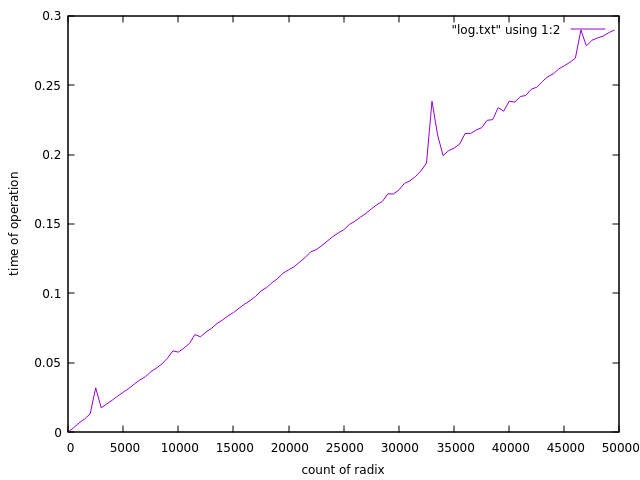
\includegraphics[scale=0.5]{../plots/onsf.png}
  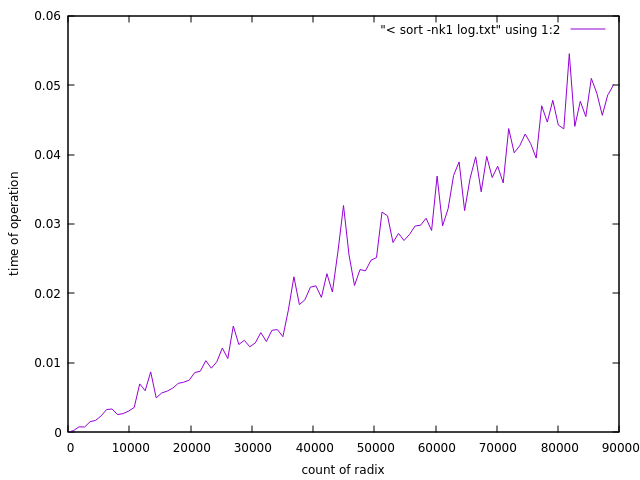
\includegraphics[scale=0.5]{../plots/onsf2.png}
  \caption{Зависимость времени построения дерева от длины текста до и после исправления}
\end{figure}


\begin{figure}[h]
  \begin{center}
    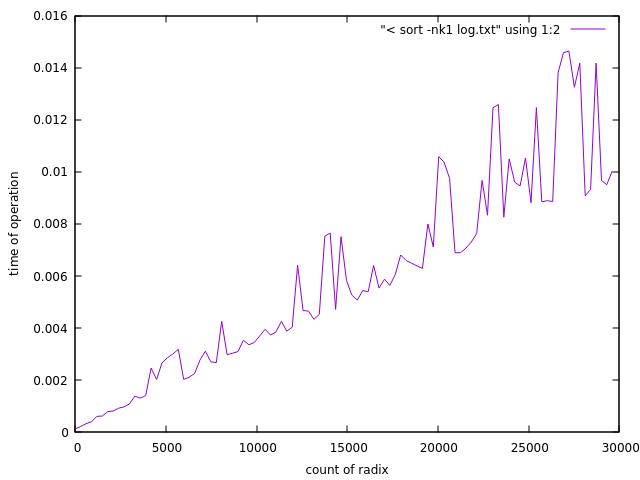
\includegraphics[scale = 0.5]{../plots/find.png}
  \end{center}
  \caption{Зависимость времени поиска от длины паттерна}
\end{figure}


\pagebreak
